\documentclass[compress,mathserif,cjk]{beamer}
\usepackage{mathrsfs}
\usepackage{color}
\usepackage{CJK}
\usepackage{amssymb}
\usepackage{amsmath}
\usepackage{extarrows}
\usepackage{ulem}
\usepackage{latexsym}
\usepackage{pmat}

% Copyright 2003 by Till Tantau <tantau@cs.tu-berlin.de>.
%
% This program can be redistributed and/or modified under the terms
% of the LaTeX Project Public License Distributed from CTAN
% archives in directory macros/latex/base/lppl.txt.

%
% The purpose of this example is to show how \part can be used to
% organize a lecture.
%
\usetheme{Warsaw}
  % 可供选择的主题参见 beameruserguide.pdf, 第 134 页起
  % 无导航条的主题: Bergen, Boadilla, Madrid, Pittsburgh, Rochester;
  % 有树形导航条的主题: Antibes, JuanLesPins, Montpellier;
  % 有目录竖条的主题: Berkeley, PaloAlto, Goettingen, Marburg, Hannover;
  % 有圆点导航条的主题: Berlin, Dresden, Darmstadt, Frankfurt, Singapore, Szeged;
  % 有节与小节导航条的主题: Copenhagen, Luebeck, Malmos, Warsaw

%  \setbeamercovered{transparent}
% 如果取消上一行的注解 %, 就会使得被覆盖部分变得透明(依稀可见)

\usepackage[english]{babel}
\usepackage[latin1]{inputenc}
\usepackage{CJK}

%\usepackage{beamerthemesplit}
%\usepackage{beamerthemeshadow,color}
\usepackage{pgf,pgfarrows,pgfnodes,pgfautomata,pgfheaps,pgfshade}
\usepackage{amsmath,amssymb}
\usepackage{bm}
\usepackage{colortbl}

\graphicspath{{images/}}         %% 图片路径. 本文的图片都放在这个文件夹里了.
\DeclareGraphicsRule{*}{mps}{*}{} %% 使 pdflatex 可以纳入 metapost 做的图片.
\renewcommand{\div}{\operatorname{div}}
\renewcommand{\raggedright}{\leftskip=0pt \rightskip=0pt plus 0cm}
\raggedright %% 中文对齐

%==============自定义: 逐个 item 高亮(\hilite), 或"高黑"(\hidark)==================%
\def\hilite<#1>{%
\temporal<#1>{\color{blue!35}}{\color{magenta}}%
{\color{blue!75}}}
\def\hidark<#1>{%
\temporal<#1>{\color{black!35}}{\color{magenta}}%
{\color{black}}}

\newcolumntype{H}{>{\columncolor{blue!20}}c!{\vrule}}
\newcolumntype{H}{>{\columncolor{blue!20}}c}  %% 表格设置
%==================================参考文献==============================================================
\newcommand{\upcite}[1]{\textsuperscript{\cite{#1}}}  %自定义命令\upcite, 使参考文献引用以上标出现
\bibliographystyle{plain}
%=========================================================================================

\def\colorb{\textcolor[rgb]{0.00,0.00,1.00}}
\def\colorg{\textcolor[rgb]{0.00,1.00,0.00}}
\def\colorr{\textcolor[rgb]{1.00,0.00,0.00}}
\newcommand\hdim{\dim_{\mathrm H}}
\newtheorem{lem}{Lemma}[section]
\newtheorem{nt}[lem]{Notation}
\newtheorem{dfn}[lem]{Definition}
\newtheorem{pro}[lem]{Proposition}
\newtheorem{thm}[lem]{Theorem}
\newtheorem{exa}[lem]{Example}
\newtheorem{cor}[lem]{Corollary}
\theoremstyle{remark}
\newtheorem*{rem}{Remark}
\numberwithin{equation}{section}
\def\N{\mathbb N}
\def\Q{\mathbb Q}
\def\R{\mathbb R}
\def\Z{\mathbb Z}
\def\vep{\varepsilon}
%=========================================================================================
%\setbeamercovered{transparent}
%
% The following info should normally be given in you main file:
%

%%%%%%%%%%%%%%%%%%%%%%%%%%%%%%%%%%%%%%%%%%%%%%%%%%%%%%%%%%%%%%%%%%%%%%%%%%%%%%%%%%%%%%%%%%%%%%%%%%%%%%%%%
%                                           定制幻灯片---重定义字体、字号命令                           %
%%%%%%%%%%%%%%%%%%%%%%%%%%%%%%%%%%%%%%%%%%%%%%%%%%%%%%%%%%%%%%%%%%%%%%%%%%%%%%%%%%%%%%%%%%%%%%%%%%%%%%%%%
\newcommand{\song}{\CJKfamily{song}}    % 宋体   (Windows自带simsun.ttf)
\newcommand{\fs}{\CJKfamily{fs}}        % 仿宋体 (Windows自带simfs.ttf)
\newcommand{\kai}{\CJKfamily{kai}}      % 楷体   (Windows自带simkai.ttf)
\newcommand{\hei}{\bf}      % 黑体   (Windows自带simhei.ttf)
\newcommand{\li}{\CJKfamily{li}}        % 隶书   (Windows自带simli.ttf)
\newcommand{\you}{\CJKfamily{you}}      % 幼圆   (Windows自带simyou.ttf)
\newcommand{\chuhao}{\fontsize{42pt}{\baselineskip}\selectfont}     % 字号设置
\newcommand{\xiaochuhao}{\fontsize{36pt}{\baselineskip}\selectfont} % 字号设置
\newcommand{\yichu}{\fontsize{32pt}{\baselineskip}\selectfont}      % 字号设置
\newcommand{\yihao}{\fontsize{28pt}{\baselineskip}\selectfont}      % 字号设置
\newcommand{\erhao}{\fontsize{21pt}{\baselineskip}\selectfont}      % 字号设置
\newcommand{\xiaoerhao}{\fontsize{18pt}{\baselineskip}\selectfont}  % 字号设置
\newcommand{\sanhao}{\fontsize{15.75pt}{\baselineskip}\selectfont}  % 字号设置
\newcommand{\sihao}{\fontsize{14pt}{\baselineskip}\selectfont}      % 字号设置
\newcommand{\xiaosihao}{\fontsize{12pt}{\baselineskip}\selectfont}  % 字号设置
\newcommand{\wuhao}{\fontsize{10.5pt}{\baselineskip}\selectfont}    % 字号设置
\newcommand{\xiaowuhao}{\fontsize{9pt}{\baselineskip}\selectfont}   % 字号设置
\newcommand{\liuhao}{\fontsize{7.875pt}{\baselineskip}\selectfont}  % 字号设置
\newcommand{\qihao}{\fontsize{5.25pt}{\baselineskip}\selectfont}    % 字号设置

%======================= 标题名称中文化 ============================%
\newtheorem{dingyi}{\hei 定义~}[section]
\newtheorem{dingli}{\hei 定理~}[section]
\newtheorem{yinli}[dingli]{\hei 引理~}
\newtheorem{tuilun}[dingli]{\hei 推论~}
\newtheorem{mingti}[dingli]{\hei 命题~}
%%%%%%%%%%%%%%%%%%%%%%%%%%%%%%%%%%%%%%%%%%%%%%%%%%%%%%%%%%%%%%%%%%%%%%%%%%%%%%%%%%%%%%%

% \usepackage{beamerthemesplit} // Activate for custom appearance


\title{\textsc{第0章\ \ \ 预备知识}}
\author{郑州大学数学与统计学院 线性代数教研室}
\date{}

\begin{document}
\begin{CJK}{UTF8}{gbsn}
\frame{\titlepage}

\begin{frame}\frametitle{目录}
 \tableofcontents
\end{frame}
%%%%%%%%%%%%%%%%%%%%%%%%%%%%%%%%%%%%%%%%%%%%%%%%%%%%%%%%%%%%%%%%%%%%%%%%%%%%%%%%%%%%%%

%%%%%%%%%%%%%%%%%%%%%%%%%%%%%%%%%%%%%%%%%%%%%%%%%%%%%%%%%%%%%%%%%%%%%%%%%%%%%%%%%%%%%%

\section[0.1]{0.1 复数\ \ 数域}
\begin{frame}{复数}

 \ \ \ \ {\hei 定义~0.1} 设$a,b$为实数, i为虚数单位满足$\mathrm i^2=-1$, 则称$z=a+b\mathrm i$为一个{\hei 复数}, 其中$a,b$分别为$z$的{\hei 实部、虚部}。
 \pause\vskip5pt
 \ \ \ \ 复数$z=a+b\mathrm i$和$w=c+d\mathrm i$的和、差、积、商分别为\pause
 $$z\pm w=(a\pm c)+(b\pm d)\mathrm i,$$
 $$zw=(ac-bd)+(bc+ad)\mathrm i.$$
 如果$c+d\mathrm i\neq0$, 即$c^2+d^2\neq0$, 则
 $$\frac{z}w\pause=\frac{a+b\mathrm i}{c+d\mathrm i}=\frac{(a+b\mathrm i)(c-d\mathrm i)}{(c+d\mathrm i)(c-d\mathrm i)}=\frac{(ac+bd)+(bc-ad)\mathrm i}{c^2+d^2}.$$
\end{frame}

\begin{frame}
 \ \ \ \ 根据定义,复数$z=a+b\mathrm i$有两种情况:$\left\{\begin{array}{ll}b=0, &\mbox{实数}\\b\neq0,&\mbox{虚数}\end{array}\right.$, 特别地,$a=0,b\neq0$时称为纯虚数。
\end{frame}

\begin{frame}{共轭复数和模}
\ \ \ \ {\hei 定义~0.2} 复数$z=a+b\mathrm i$的{\hei 共轭复数}为$\bar z=a-b\mathrm i$
\pause\vskip5pt
 \ \ \ \ 共轭复数有如下性质:
 $$\bar{\bar z}=z,\ \ \overline{z\pm w}=\bar z\pm\bar w,\ \ \overline{zw}=\bar z\bar w,\ \ \overline{\Big(\frac{z}w\Big)}=\frac{\bar z}{\bar w}~~(w\neq0).$$
 特别地,$z$为实数$\Longleftrightarrow~z=\bar z$,~~~~$z$为纯虚数$\Longleftrightarrow~z=-\bar z$.
 \pause\vskip10pt
 \ \ \ \ {\hei 定义~0.3} 复数$z=a+b\mathrm i$的{\hei 模}为$|z|=\sqrt{a^2+b^2}$.
 \pause\vskip5pt
 \ \ \ \ 显然有\\
 \hspace{6em}$|z|^2=z\bar z,~~~~~~~~~~~|\bar z|=|z|,~~~~~~~~~~~~~~~$\\
 \hspace{5em}$|zw|=|z||w|,~~~\Big|\frac{z}w\Big|=\frac{|z|}{|w|}~~(w\neq0),$\\
 \hspace{6em} $|z|-|w|\leq|z+w|\leq |z|+|w|.$\\
 因此模与绝对值相容。
\end{frame}

\begin{frame}{复数的坐标表示}

 $z=a+b\mathrm i~\longleftrightarrow~\mbox{有序实数对}(a,b)~\longleftrightarrow~\mbox{坐标平面中的点}~\longleftrightarrow~\mbox{向量}$
 \pause
 \begin{figure}[!h]
  \centering
  % Requires \usepackage{graphicx}
  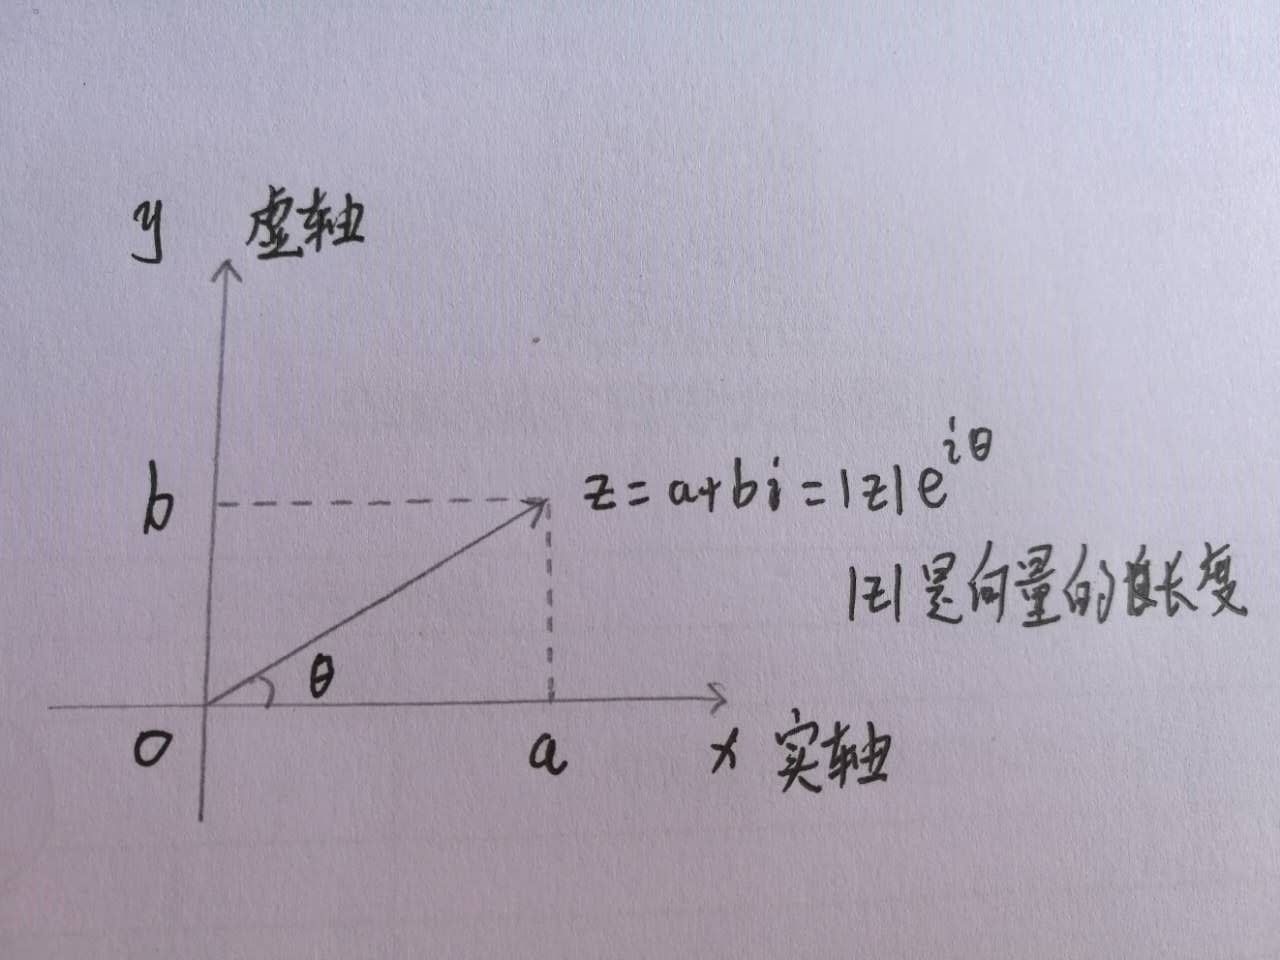
\includegraphics[width=2.5in]{f0-1}
 \end{figure}
 \ \ \ \ $\theta$称为$z$的辐角,辐角为$\theta$的单位向量对应的复数记为$\mathrm e^{i\theta}=\cos\theta+\mathrm i\sin\theta$, 则$z=|z|\mathrm e^{i\theta}$.
\end{frame}

\begin{frame}
 \ \ \ \ 若$z=|z|\mathrm e^{i\theta},~w=|w|\mathrm e^{i\phi}$, 则
 $$zw\pause=|z|\mathrm e^{i\theta}|w|\mathrm e^{i\phi}=|z||w|\mathrm e^{i(\theta+\phi)}.$$
 特别地,$z^n=|z|^n\mathrm e^{\mathrm in\theta}$.
 \pause\vskip10pt
 \ \ \ \ 数集的一些记号:\\
 \ \ \ \ 自然数集$\mathbf N$, 整数集$\mathbf Z$, 有理数集$\mathbf Q$, 实数集$\mathbf R$, 复数集$\mathbf C$.


\end{frame}

\begin{frame}{代数学基本定理}
 \ \ \ \ $n$次复系数多项式一般具有如下形式:
 $$f(x)=a_0+a_1x+a_2x^2+\cdots+a_nx^n,~~~~a_i\in\mathbf C$$
 \pause\vskip5pt
 \ \ \ \ {\hei 代数学基本定理} 任意一个正次数的复系数多项式都至少有一个复数根。
 \pause\vskip15pt
 \ \ \ \ {\hei 推论} 设$f(x)$是一个$n~(n>0)$次复系数多项式,则存在复数$c_1,c_2,\cdots,c_n$ 使$f(x)=k(x-c_1)(x-c_2)\cdots(x-c_n)$, 其中$k$为$f(x)$中$x^n$的系数。
\end{frame}

\begin{frame}{数域}
 \ \ \ \ {\hei 定义~0.4} 设$P\subseteq\mathbf C$, 如果对$P$中任意两个数作某种运算,其结果仍在$P$中,则称$P$对该运算{\hei 封闭}。
 \pause\vskip10pt
 \ \ \ \ 显然,$\mathbf{Q,R,C}$对加、减、乘、除(除数不为0)都是封闭的,$\mathbf Z$对加、减、乘运算封闭,但对除法(除数不为0)不封闭。
  \pause\vskip10pt
  \ \ \ \ {\hei 定义~0.5} 设$P\subseteq\mathbf C$且$0,1\in P$, 如果$P$对加、减、乘、除(除数不为0)都是封闭的,则称$P$为一个{\hei 数域}。
  \pause\vskip10pt
  \ \ \ \ 因此,$\mathbf{Q,R,C}$都是数域,而$\mathbf Z$和无理数集不构成数域。
  \pause\vskip10pt
  \ \ \ \ {\hei 例~1} 证明$\mathbf Q(\sqrt{2})=\{a+b\sqrt2~|~a,b\in\mathbf Q\}$是一个数域。
  \pause\vskip10pt
  \ \ \ \ {\hei 证明} 显然$0,1\in\mathbf Q(\sqrt{2})$, 剩下只需表明$\mathbf Q(\sqrt2)$对加、减、乘、除(除数不为0)都封闭即可。$\hfill\Box$
\end{frame}

\begin{frame}

 \ \ \ \ {\hei 定理~0.1} 任意一个数域$P$都包含有理数域$\mathbf Q$, 因此$\mathbf Q$是最小的数域。
 \pause\vskip10pt
  \ \ \ \ {\hei 证明} 首先有$0,1\in P$, $\because P$对加法和减法封闭,$\therefore\forall n\in\mathbf Z^+$有
  $$n=1+1+\cdots+1\in P,~~~-n=0-n\in P.$$
  $\therefore\mathbf Z\subseteq P$.
  \pause\vskip5pt
  \ \ \ \ 已知有理数$a$都可以写成$\frac{m}n~(m,n\in Z,n\neq0)$的形式,由$P$对除法的封闭性可知$a\in P$, 即$\mathbf Q\subseteq P.\hfill\Box$
\end{frame}

\section[0.2]{0.2 二、三阶行列式}
\begin{frame}{二阶行列式}
 \ \ \ \ 设
 $$\left\{\begin{array}{l}
 a_{11}x_1+a_{12}x_2=b_1,\\
 a_{21}x_1+a_{22}x_2=b_2,
 \end{array}\right.$$
 当$a_{11}a_{22}-a_{12}a_{21}\neq0$时,其一般解为
 $$x_1=\frac{b_1a_{22}-b_2a_{12}}{a_{11}a_{22}-a_{12}a_{21}},~~~~x_2=\frac{b_2a_{11}-b_1a_{21}}{a_{11}a_{22}-a_{12}a_{21}}.$$
 \pause
  引入符号$D=\left|\begin{matrix}a_{11}&a_{12}\\a_{21}&a_{22}\end{matrix}\right|=a_{11}a_{22}-a_{12}a_{21}$, 称为{\hei 二阶行列式}。 \pause 令
  $$D_1=\left|\begin{matrix}b_1&a_{12}\\b_2&a_{22}\end{matrix}\right|=b_1a_{22}-b_2a_{12},~~~~D_2=\left|\begin{matrix}a_{11}&b_1\\a_{21}&b_2\end{matrix}\right|=a_{11}b_2-a_{21}b_1,$$
  于是其解可表示为
  $$x_1=\frac{D_1}D,~~~~x_2=\frac{D_2}D.$$
\end{frame}

\begin{frame}{三阶行列式}
 \ \ \ \ 同样在三元一次线性方程组
 $$\left\{\begin{array}{l}
 a_{11}x_1+a_{12}x_2+a_{13}x_3=b_1,\\
 a_{21}x_1+a_{22}x_2+a_{23}x_3=b_2,\\
 a_{31}x_1+a_{32}x_2+a_{33}x_3=b_3,
 \end{array}\right.$$
 中引入符号
 $$\begin{array}{l}
 D=\left|\begin{matrix}a_{11}&a_{12}&a_{13}\\a_{21}&a_{22}&a_{23}\\a_{31}&a_{32}&a_{33}\end{matrix}\right|
   \begin{matrix}\\~~=~~~a_{11}a_{22}a_{33}+a_{12}a_{23}a_{31}+a_{13}a_{21}a_{32}\\~~~~~~-a_{11}a_{23}a_{32}-a_{12}a_{21}a_{33}-a_{13}a_{22}a_{31}\end{matrix}\\\\
 \pause\hspace{6em}=a_{11}\left|\begin{matrix}a_{22}&a_{23}\\a_{32}&a_{33}\end{matrix}\right|-a_{12}\left|\begin{matrix}a_{21}&a_{23}\\a_{31}&a_{33}\end{matrix}\right|
          +a_{13}\left|\begin{matrix}a_{21}&a_{22}\\a_{31}&a_{32}\end{matrix}\right|
 \end{array}$$
 称为{\hei 三阶行列式}。
\end{frame}

\begin{frame}
并令
$$D_1=\left|\begin{matrix}b_1&a_{12}&a_{13}\\b_2&a_{22}&a_{23}\\b_3&a_{32}&a_{33}\end{matrix}\right|,~~~~
D_2=\left|\begin{matrix}a_{11}&b_1&a_{13}\\a_{21}&b_2&a_{23}\\a_{31}&b_3&a_{33}\end{matrix}\right|,~~~~
D_3=\left|\begin{matrix}a_{11}&a_{12}&b_1\\a_{21}&a_{22}&b_2\\a_{31}&a_{32}&b_3\end{matrix}\right|.$$
当$D\neq0$, 则其解可表示为
$$x_1=\frac{D_1}D,~~~~x_2=\frac{D_2}D,~~~~x_3=\frac{D_3}D.$$
\end{frame}

\begin{frame}{例题}
\ \ \ \ {\hei 例~1} 求解二元一次方程组
$$\left\{\begin{array}{rcl}
2x_1-x_2&=&5,\\3x_1+2x_2&=&11.
\end{array}\right.$$
 \pause\vskip5pt
 \ \ \ \ {\hei 例~2} 求解
 $$\left\{\begin{array}{rcl}
 2x_1-x_2+3x_3&=&9,\\x_1-2x_2-x_3&=&-6,\\4x_1+x_2+2x_3&=&12.
 \end{array}\right.$$
\end{frame}


%=====================================================frame8=========================================


\begin{frame}
\begin{center}
{\textcolor[rgb]{0.50,0.00,1.00}{\textbf{\xiaoerhao{Thanks for your attention!}}}}\bigskip
\end{center}
\end{frame}
\end{CJK}
\end{document}


